\documentclass[12pt]{article}
\usepackage{fullpage}
\usepackage{amsmath, amsthm, amssymb}
\usepackage{enumerate}
\usepackage{mathtools}

\usepackage[usenames,dvipsnames]{xcolor}
\usepackage{tkz-graph}
\usetikzlibrary{arrows}

\newtheorem*{claim}{Claim}
\newtheorem{lemma}{Lemma}
\newtheorem{theorem}{Theorem}
\newtheorem*{definition}{Definition}
\begin{document}
\title{INFO 4220 Homework 3}
\author{Dominick Twitty}
\date{}
\maketitle
\section{Pareto Improvements}
\begin{enumerate}[(a)]
\item Given a matching $M_2$, which is a Pareto improvement of a matching $M_1$, the only way to determine the Pareto-efficiency of $M_2$ is to compare it to all other possible matchings. If there exist other matchings besides $M_1$ and $M_2$, we need more information.  If $M_1$ and $M_2$ are the only matchings, then $M_2$ is Pareto-efficient.

\item Suppose we have a matching $M$ with an augmenting path. We know this means that $M$ is not a maximum matching. Given this path, we can generate a matching $M'$ with one more edge than $M$ that contains at least every vertex that $M$ contains (and thus Pareto-dominates $M$). Along the path $P$, for $e \in P$, if $e \in M$, set $e \notin M'$, and if $e \notin M$, set $e \in M$. The vertices at the start and end of the path will now be in the matching, and thus will be strictly better off. For every vertex in between, we remove one of its edges from the matching, but then add another, so every intermediate vertex will not be worse off. All other vertices not in $P$ are unaffected. $M'$ now has every vertex at least as well off, with two vertices strictly improved. Therefore, if $M$ contains an augmenting path, $M$ cannot be Pareto-optimal.

\item 
\begin{enumerate}[i.]
\item There are no possible Pareto-improvements in this situation. The only other possible matching is $\{(a, y), (b, x)\}$, which would leave $a$ worse off.
\item The matching $M_1$ is not Pareto-efficient. The matching $M_2 = \{(a, z), (b, x), (c, y)\}$ gives a strictly better assignment to all three agents, and therefore $M_2$ Pareto-dominates $M_1$.
\end{enumerate}

\item 
We assume that the matching $M$ given is complete (no agent or house is unassigned). Given a set of agents $A = a_1,\ldots,a_n$, with each $a_i$ with a set of preferences $\succ_{a_i}$, and a set of houses $H = h_1,\ldots h_n$. Let all agents and houses be considered interchangeably with vertices of a bipartite graph $\hat{G}$. We add an edge between agent $a$ and house $h$ with weight $\texttt{index}(\succ_a, h)$. That is, if $h$ is first in $\succ_a$, add an edge $(a, h)$ with weight 1. If $h$ is second, add an edge with weight 2, etc.

We define a \emph{rotation path} $P$ as a cycle in $\hat{G}$ with the property that for each agent $a$ in $P$, the edges $e = (a, M(a))$ and $e' = (a, M'(a) \neq M(a))$ are in $P$, with weights $w(e') < w(e)$. One can see that every agent in the cycle prefers another's house to their own.

\begin{claim}
A matching $M$ is Pareto-efficient if and only if there does not exist a rotation path in $\hat{G}(M)$.
\end{claim}
\begin{proof}
We prove both directions.
\begin{description}
\item[$\implies$] Suppose $\hat{G}$ contains a rotation path $P$ where every agent $a$ in $P$ prefers $M'(a)$ to their current assignment $M(a)$. As $P$ is a cycle, clearly there is some $b$ in $P$ such that $b$ prefers $M(a)$ to $M(b)$ ($M'(b) = M(a)$). This property continues throughout $P$ until $M'(a) = M(c)$ for some $c$ in $P$. If one were to reassign every $a$ to $M'(a)$ (the ``rotation'' we speak of), every agent in $P$ would strictly benefit, and every agent not in $P$ would see no change. Therefore, the resultant matching $M'$ would Pareto-dominate $M$ and we can say that $M$ is not Pareto-efficient.

\item[$\impliedby$] We assume $M$ is not Pareto-efficient, and that there is no rotation path in $\hat{G}(M)$.  Because any reallocation implies changing the assignments of at least two agents, this means that no set of agents strictly benefits by swapping houses. This must hold for all subsets of $A$. If no subset of $A$ can benefit by swapping, then no agent can strictly benefit without hurting another agent. This means $M$ is Pareto-efficient, and we have a contradiction. Therefore, the absence of a rotation path implies that $M$ is Pareto-efficient.
\end{description}
\end{proof}

\item Find below the graph we generate from the previous example, with the given matched edges in bold. Edge weight labels in a full bipartite graph are tricky, so I had to make the graph beautiful. The rotation path is $\{(a, x), (a, z), (c, z), (c, y), (b, y), (b,x)\}$. As claimed, rotating houses produces the Pareto-improved matching $\{(a, z), (b, x), (c, y)\}$.
\end{enumerate}
\SetVertexNormal[Shape      = circle,
                 FillColor  = orange,
                 LineWidth  = 2pt]
\SetUpEdge[lw         = 1.5pt,
           color      = black,
           labelcolor = white,
           labeltext  = red,
           labelstyle = {sloped,draw,text=blue}]
\begin{center}
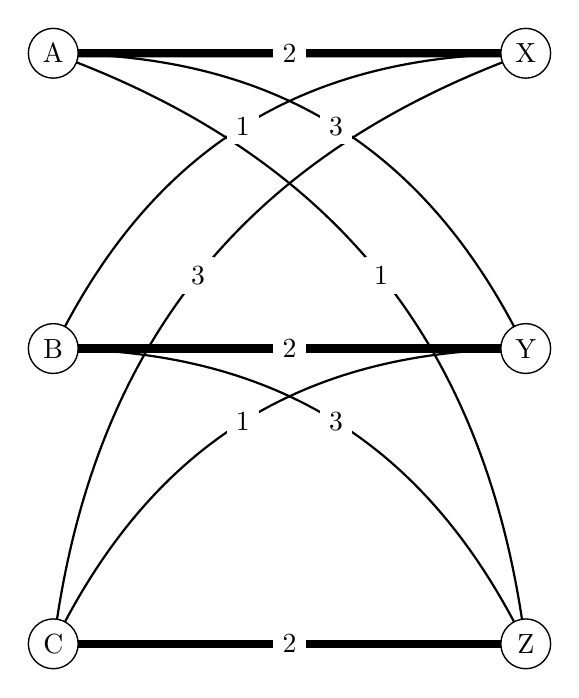
\begin{tikzpicture}[scale = 0.75]
\Vertex[x=0 ,y=10]{A}
\Vertex[x=0 ,y=5]{B}
\Vertex[x=0, y=0]{C}
\Vertex[x=8 ,y=10]{X}
\Vertex[x=8 ,y=5]{Y}
\Vertex[x=8 ,y=0]{Z}

\Edge[label = $2$, lw = 3.0pt](A)(X)
\Edge[label = $2$, lw = 3.0pt](B)(Y)
\Edge[label = $2$, lw = 3.0pt](C)(Z)
\tikzset{EdgeStyle/.append style = {bend left}}
\Edge[label = $1$](C)(Y)
\Edge[label = $3$](B)(Z)
\Edge[label = $3$](C)(X)
\Edge[label = $1$](A)(Z)
\Edge[label = $1$](B)(X)
\Edge[label = $3$](A)(Y)
\end{tikzpicture}
\end{center}

\section{Markets with Mixed Initial Endowments}
\begin{enumerate}[(a)]
\item When Charlie ignores initial endowments, he can no longer guarantee that second-years will get at least as good an assignment as they did last year.

\item 
\begin{enumerate}[i.]
\item While the mechanism is Pareto-efficient with regards to participating students, it is not Pareto-efficient with regards to the total set of students and rooms. Consider the following situation. There are two students, $a$ and $b$, and two rooms, $x$ and $y$. There is an initial endowment where $a$ holds $x$. The preference lists are
\begin{align*}
a &: y \succ x & b &: x \succ y
\end{align*}

As is her right, $a$ opts out. The only possible matching now is $M = \{(a, x),  (b, y)\}$. With regards to the total input set, $M$ is not Pareto-efficient. The matching $M' = \{(a, y),  (b, x)\}$ Pareto-dominates $M$. Therefore, the mechanism is not Pareto-efficient.

\item Firstly, opt-outs cannot gain or lose anything by lying about preferences, so the mechanism is strategyproof for opt-outs. The sub-market formed by removing opt-outs from the original market is no different from any other market (just a bit smaller). The serial dictatorship is strategyproof on arbitrary complete markets. Therefore, the serial dictatorship is strategyproof on the sub-market of those who choose to participate.
\end{enumerate}

\item 
\begin{enumerate}[i.]
\item The given application of the TTC algorithm is individually rational. The TTC algorithm is guaranteed to give each participant a match at least as good as their initial endowment. For second-years, this holds. For new students, the initial endowment is no room, and with the assumption that any room is better than no room, any output matching is better than not participating. Therefore, the mechanism is individually rational.

\item As the TTC algorithm produces a core matching in any trading market with strict rank ordering, the matching produced by this mechanism will be Pareto-efficient.
\end{enumerate}
\end{enumerate}

\section{Weak Preferences in Markets with Initial Endowments}
\begin{enumerate}[(a)]
\item The core matching in this market, computed via the TTC algorithm, is $\{(a, h_c), (b, h_b), (c, h_a)\}$.
\item There is no core matching. In all Pareto-efficient and individually rational matchings, there exists a pair that can leave the market and trade with each other.
\item The modified TTC algorithm is not Pareto-efficient. The arbitrary removal of intersecting cycles is the same as applying an arbitrary strict ordering on a weak order. Consider the weak-preference example from part 2. If the modified TTC algorithm selects the ordering used in part 1, it will return the matching $\{(a, h_c), (b, h_b), (c, h_a)\}$. However, in this matching, if $a$ and $b$ switch (forming the matching $\{(a, h_b), (b, h_c), (c, h_a)\}$), $a$ is unchanged and $b$ strictly benefits.
\end{enumerate}
\end{document}
